It is well-known that imbalance in trees leads to degradation in performance;
for instance, a $kd$-tree node with every descendant except one in its left
child is effectively useless.  A $kd$-tree full of nodes like this will perform
abysmally for nearest neighbor search, and it is not hard to generate a dataset
that will cause a $kd$-tree of this sort.

This sort of imbalance applies to all types of trees, not just $kd$-trees.  In
our situation, we are interested in a better understanding of this imbalance for
cover trees, and thus endeavor to introduce a more formal measure of imbalance
which is correlated with tree performance.  Numerous measures of tree
imbalance have already been established; one example is that proposed by
\citet{colless1982review}, and another is Sackin's index \citep{sackin1972good},
but we aim to capture a different measure of imbalance that utilizes the leveled
structure of the cover tree.

We already know each node in a cover tree is indexed with an integer level (or
scale).  In the explicit representation of the cover tree, each non-leaf node
has children at a lower level.  But these children need not be strictly one
level lower; see Figure \ref{fig:imbalance}.  In Figure
\ref{fig:imbalance-good}, each cover tree node has children that are strictly
one level lower; we will refer to this as a {\em perfectly balanced cover tree}.
Figure \ref{fig:imbalance-bad}, on the other hand, contains the node
$\mathscr{N}_m$ which has two children with scale two less than $s_m$.  We will
refer to this as an {\em imbalanced cover tree}.  Note that in our definition,
the balance of a cover tree has nothing to do with differing number of
descendants in each child branch but instead only missing levels.

\begin{figure}
\begin{subfigure}[b]{0.585\textwidth}
  \begin{center}
    
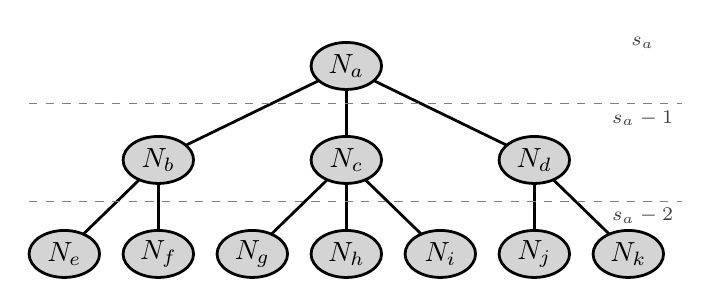
\begin{tikzpicture}[>=latex,line join=bevel,scale=0.47]
  \pgfsetlinewidth{1bp}
%%
\begin{scope}
  \pgfsetstrokecolor{black}
  \definecolor{strokecol}{rgb}{1.0,1.0,1.0};
  \pgfsetstrokecolor{strokecol}
  \definecolor{fillcol}{rgb}{1.0,1.0,1.0};
  \pgfsetfillcolor{fillcol}
  \filldraw (0bp,0bp) -- (0bp,180bp) -- (486bp,180bp) -- (486bp,0bp) -- cycle;
\end{scope}
\begin{scope}
  \pgfsetstrokecolor{black}
  \definecolor{strokecol}{rgb}{1.0,1.0,1.0};
  \pgfsetstrokecolor{strokecol}
  \definecolor{fillcol}{rgb}{1.0,1.0,1.0};
  \pgfsetfillcolor{fillcol}
  \filldraw (0bp,0bp) -- (0bp,180bp) -- (486bp,180bp) -- (486bp,0bp) -- cycle;
\end{scope}
\begin{scope}
  \pgfsetstrokecolor{black}
  \definecolor{strokecol}{rgb}{1.0,1.0,1.0};
  \pgfsetstrokecolor{strokecol}
  \definecolor{fillcol}{rgb}{1.0,1.0,1.0};
  \pgfsetfillcolor{fillcol}
  \filldraw (0bp,0bp) -- (0bp,180bp) -- (486bp,180bp) -- (486bp,0bp) -- cycle;
\end{scope}
  \pgfsetcolor{black}
  % Edge: c2 -> c6
  \draw [-] (228.43bp,74.834bp) .. controls (218.25bp,64.938bp) and (204.48bp,51.546bp)  .. (185.8bp,33.385bp);
  % Edge: c3 -> c9
  \draw [-] (387bp,71.697bp) .. controls (387bp,63.983bp) and (387bp,54.712bp)  .. (387bp,36.104bp);
  % Edge: c3 -> c10
  \draw [-] (401.57bp,74.834bp) .. controls (411.75bp,64.938bp) and (425.52bp,51.546bp)  .. (444.2bp,33.385bp);
  % Edge: c2 -> c8
  \draw [-] (257.57bp,74.834bp) .. controls (267.75bp,64.938bp) and (281.52bp,51.546bp)  .. (300.2bp,33.385bp);
  % Edge: c1 -> c4
  \draw [-] (84.43bp,74.834bp) .. controls (74.25bp,64.938bp) and (60.476bp,51.546bp)  .. (41.796bp,33.385bp);
  % Edge: c1 -> c5
  \draw [-] (99bp,71.697bp) .. controls (99bp,63.983bp) and (99bp,54.712bp)  .. (99bp,36.104bp);
  % Edge: root -> c1
  \draw [-] (221.75bp,150.67bp) .. controls (197.4bp,138.83bp) and (157.28bp,119.33bp)  .. (120.33bp,101.37bp);
  % Edge: root -> c2
  \draw [-] (243bp,143.7bp) .. controls (243bp,135.98bp) and (243bp,126.71bp)  .. (243bp,108.1bp);
  % Edge: c2 -> c7
  \draw [-] (243bp,71.697bp) .. controls (243bp,63.983bp) and (243bp,54.712bp)  .. (243bp,36.104bp);
  % Edge: root -> c3
  \draw [-] (264.25bp,150.67bp) .. controls (288.6bp,138.83bp) and (328.72bp,119.33bp)  .. (365.67bp,101.37bp);
  % Node: c7
\begin{scope}
  \definecolor{strokecol}{rgb}{0.0,0.0,0.0};
  \pgfsetstrokecolor{strokecol}
  \definecolor{fillcol}{rgb}{0.83,0.83,0.83};
  \pgfsetfillcolor{fillcol}
  \filldraw [opacity=1] (243bp,18bp) ellipse (27bp and 18bp);
  \draw (243bp,18bp) node {$\mathscr{N}_h$};
\end{scope}
  % Node: c9
\begin{scope}
  \definecolor{strokecol}{rgb}{0.0,0.0,0.0};
  \pgfsetstrokecolor{strokecol}
  \definecolor{fillcol}{rgb}{0.83,0.83,0.83};
  \pgfsetfillcolor{fillcol}
  \filldraw [opacity=1] (387bp,18bp) ellipse (27bp and 18bp);
  \draw (387bp,18bp) node {$\mathscr{N}_j$};
\end{scope}
  % Node: c8
\begin{scope}
  \definecolor{strokecol}{rgb}{0.0,0.0,0.0};
  \pgfsetstrokecolor{strokecol}
  \definecolor{fillcol}{rgb}{0.83,0.83,0.83};
  \pgfsetfillcolor{fillcol}
  \filldraw [opacity=1] (315bp,18bp) ellipse (27bp and 18bp);
  \draw (315bp,18bp) node {$\mathscr{N}_i$};
\end{scope}
  % Node: c3
\begin{scope}
  \definecolor{strokecol}{rgb}{0.0,0.0,0.0};
  \pgfsetstrokecolor{strokecol}
  \definecolor{fillcol}{rgb}{0.83,0.83,0.83};
  \pgfsetfillcolor{fillcol}
  \filldraw [opacity=1] (387bp,90bp) ellipse (27bp and 18bp);
  \draw (387bp,90bp) node {$\mathscr{N}_d$};
\end{scope}
  % Node: c2
\begin{scope}
  \definecolor{strokecol}{rgb}{0.0,0.0,0.0};
  \pgfsetstrokecolor{strokecol}
  \definecolor{fillcol}{rgb}{0.83,0.83,0.83};
  \pgfsetfillcolor{fillcol}
  \filldraw [opacity=1] (243bp,90bp) ellipse (27bp and 18bp);
  \draw (243bp,90bp) node {$\mathscr{N}_c$};
\end{scope}
  % Node: c1
\begin{scope}
  \definecolor{strokecol}{rgb}{0.0,0.0,0.0};
  \pgfsetstrokecolor{strokecol}
  \definecolor{fillcol}{rgb}{0.83,0.83,0.83};
  \pgfsetfillcolor{fillcol}
  \filldraw [opacity=1] (99bp,90bp) ellipse (27bp and 18bp);
  \draw (99bp,90bp) node {$\mathscr{N}_b$};
\end{scope}
  % Node: c10
\begin{scope}
  \definecolor{strokecol}{rgb}{0.0,0.0,0.0};
  \pgfsetstrokecolor{strokecol}
  \definecolor{fillcol}{rgb}{0.83,0.83,0.83};
  \pgfsetfillcolor{fillcol}
  \filldraw [opacity=1] (459bp,18bp) ellipse (27bp and 18bp);
  \draw (459bp,18bp) node {$\mathscr{N}_k$};
\end{scope}
  % Node: root
\begin{scope}
  \definecolor{strokecol}{rgb}{0.0,0.0,0.0};
  \pgfsetstrokecolor{strokecol}
  \definecolor{fillcol}{rgb}{0.83,0.83,0.83};
  \pgfsetfillcolor{fillcol}
  \filldraw [opacity=1] (243bp,162bp) ellipse (27bp and 18bp);
  \draw (243bp,162bp) node {$\mathscr{N}_a$};
\end{scope}
  % Node: c6
\begin{scope}
  \definecolor{strokecol}{rgb}{0.0,0.0,0.0};
  \pgfsetstrokecolor{strokecol}
  \definecolor{fillcol}{rgb}{0.83,0.83,0.83};
  \pgfsetfillcolor{fillcol}
  \filldraw [opacity=1] (171bp,18bp) ellipse (27bp and 18bp);
  \draw (171bp,18bp) node {$\mathscr{N}_g$};
\end{scope}
  % Node: c5
\begin{scope}
  \definecolor{strokecol}{rgb}{0.0,0.0,0.0};
  \pgfsetstrokecolor{strokecol}
  \definecolor{fillcol}{rgb}{0.83,0.83,0.83};
  \pgfsetfillcolor{fillcol}
  \filldraw [opacity=1] (99bp,18bp) ellipse (27bp and 18bp);
  \draw (99bp,18bp) node {$\mathscr{N}_f$};
\end{scope}
  % Node: c4
\begin{scope}
  \definecolor{strokecol}{rgb}{0.0,0.0,0.0};
  \pgfsetstrokecolor{strokecol}
  \definecolor{fillcol}{rgb}{0.83,0.83,0.83};
  \pgfsetfillcolor{fillcol}
  \filldraw [opacity=1] (27bp,18bp) ellipse (27bp and 18bp);
  \draw (27bp,18bp) node {$\mathscr{N}_e$};
\end{scope}
%
\draw[gray,thin,dashed] (0bp,58bp) -- (500bp,58bp);
\draw[gray,thin,dashed] (0bp,133bp) -- (500bp,133bp);

\draw (470bp,180bp) node[darkgray] {\scriptsize $s_a$};
\draw (470bp,122bp) node[darkgray] {\scriptsize $s_a - 1$};
\draw (470bp,47bp) node[darkgray] {\scriptsize $s_a - 2$};
\end{tikzpicture}


  \end{center}
  \caption{Balanced cover tree.}
  \label{fig:imbalance-good}
\end{subfigure}
\begin{subfigure}[b]{0.415\textwidth}
  \begin{center}
    
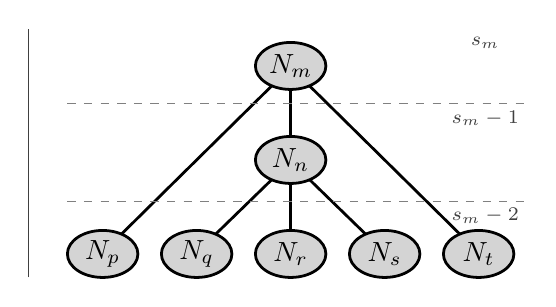
\begin{tikzpicture}[>=latex,line join=bevel,scale=0.47]
  \pgfsetlinewidth{1bp}
%%
\begin{scope}
  \pgfsetstrokecolor{black}
  \definecolor{strokecol}{rgb}{1.0,1.0,1.0};
  \pgfsetstrokecolor{strokecol}
  \definecolor{fillcol}{rgb}{1.0,1.0,1.0};
  \pgfsetfillcolor{fillcol}
  \filldraw (0bp,0bp) -- (0bp,180bp) -- (342bp,180bp) -- (342bp,0bp) -- cycle;
\end{scope}
  \pgfsetcolor{black}
  % Edge: c2 -> c6
  \draw [-] (156.43bp,74.834bp) .. controls (146.25bp,64.938bp) and (132.48bp,51.546bp)  .. (113.8bp,33.385bp);
  % Edge: root -> c4
  \draw [-] (156.4bp,146.6bp) .. controls (131.06bp,121.62bp) and (78.82bp,70.101bp)  .. (41.639bp,33.435bp);
  % Edge: c2 -> c8
  \draw [-] (185.57bp,74.834bp) .. controls (195.75bp,64.938bp) and (209.52bp,51.546bp)  .. (228.2bp,33.385bp);
  % Edge: root -> c10
  \draw [-] (185.6bp,146.6bp) .. controls (210.94bp,121.62bp) and (263.18bp,70.101bp)  .. (300.36bp,33.435bp);
  % Edge: root -> c2
  \draw [-] (171bp,143.7bp) .. controls (171bp,135.98bp) and (171bp,126.71bp)  .. (171bp,108.1bp);
  % Edge: c2 -> c7
  \draw [-] (171bp,71.697bp) .. controls (171bp,63.983bp) and (171bp,54.712bp)  .. (171bp,36.104bp);
  % Node: c7
\begin{scope}
  \definecolor{strokecol}{rgb}{0.0,0.0,0.0};
  \pgfsetstrokecolor{strokecol}
  \definecolor{fillcol}{rgb}{0.83,0.83,0.83};
  \pgfsetfillcolor{fillcol}
  \filldraw [opacity=1] (171bp,18bp) ellipse (27bp and 18bp);
  \draw (171bp,18bp) node {$\mathscr{N}_r$};
\end{scope}
  % Node: c8
\begin{scope}
  \definecolor{strokecol}{rgb}{0.0,0.0,0.0};
  \pgfsetstrokecolor{strokecol}
  \definecolor{fillcol}{rgb}{0.83,0.83,0.83};
  \pgfsetfillcolor{fillcol}
  \filldraw [opacity=1] (243bp,18bp) ellipse (27bp and 18bp);
  \draw (243bp,18bp) node {$\mathscr{N}_s$};
\end{scope}
  % Node: c2
\begin{scope}
  \definecolor{strokecol}{rgb}{0.0,0.0,0.0};
  \pgfsetstrokecolor{strokecol}
  \definecolor{fillcol}{rgb}{0.83,0.83,0.83};
  \pgfsetfillcolor{fillcol}
  \filldraw [opacity=1] (171bp,90bp) ellipse (27bp and 18bp);
  \draw (171bp,90bp) node {$\mathscr{N}_n$};
\end{scope}
  % Node: c10
\begin{scope}
  \definecolor{strokecol}{rgb}{0.0,0.0,0.0};
  \pgfsetstrokecolor{strokecol}
  \definecolor{fillcol}{rgb}{0.83,0.83,0.83};
  \pgfsetfillcolor{fillcol}
  \filldraw [opacity=1] (315bp,18bp) ellipse (27bp and 18bp);
  \draw (315bp,18bp) node {$\mathscr{N}_t$};
\end{scope}
  % Node: root
\begin{scope}
  \definecolor{strokecol}{rgb}{0.0,0.0,0.0};
  \pgfsetstrokecolor{strokecol}
  \definecolor{fillcol}{rgb}{0.83,0.83,0.83};
  \pgfsetfillcolor{fillcol}
  \filldraw [opacity=1] (171bp,162bp) ellipse (27bp and 18bp);
  \draw (171bp,162bp) node {$\mathscr{N}_m$};
\end{scope}
  % Node: c6
\begin{scope}
  \definecolor{strokecol}{rgb}{0.0,0.0,0.0};
  \pgfsetstrokecolor{strokecol}
  \definecolor{fillcol}{rgb}{0.83,0.83,0.83};
  \pgfsetfillcolor{fillcol}
  \filldraw [opacity=1] (99bp,18bp) ellipse (27bp and 18bp);
  \draw (99bp,18bp) node {$\mathscr{N}_q$};
\end{scope}
  % Node: c4
\begin{scope}
  \definecolor{strokecol}{rgb}{0.0,0.0,0.0};
  \pgfsetstrokecolor{strokecol}
  \definecolor{fillcol}{rgb}{0.83,0.83,0.83};
  \pgfsetfillcolor{fillcol}
  \filldraw [opacity=1] (27bp,18bp) ellipse (27bp and 18bp);
  \draw (27bp,18bp) node {$\mathscr{N}_p$};
\end{scope}
%
\draw[darkgray, thin] (-30bp,0bp) -- (-30bp,190bp);
\draw[gray,thin,dashed] (0bp,58bp) -- (350bp,58bp);
\draw[gray,thin,dashed] (0bp,133bp) -- (350bp,133bp);

\draw (320bp,180bp) node[darkgray] {\scriptsize $s_m$};
\draw (320bp,122bp) node[darkgray] {\scriptsize $s_m - 1$};
\draw (320bp,47bp) node[darkgray] {\scriptsize $s_m - 2$};
\end{tikzpicture}


  \end{center}
  \caption{Imbalanced cover tree.}
  \label{fig:imbalance-bad}
\end{subfigure}
\caption{Balanced and imbalanced cover trees.}
\label{fig:imbalance}
\end{figure}

An imbalanced cover tree can---and often does---happen in practice, and the
imbalance may be far worse than the simple graphs of Figure \ref{fig:imbalance}.
Consider a dataset with a single outlier which is very far away from all of the
other points\footnote{Note also that for an outlier sufficiently far away, the
expansion constant is $N - 1$.}.  Figure \ref{fig:outlier} shows what happens in
this situation: the root node has two children; one of these children has only
the outlier as a descendant, and the other child has the rest of the points in
the dataset as a descendant.  In fact, it is easy to find datasets with multiple
outliers which give rise to a chain-like structure at the top of the tree: see
Figure \ref{fig:outliers} for an illustration\footnote{As a side note, this
behavior is not limited to cover trees, and can happen to mean-split $kd$-trees
too, especially in higher dimensions.}.

\begin{figure}
\begin{center}
  
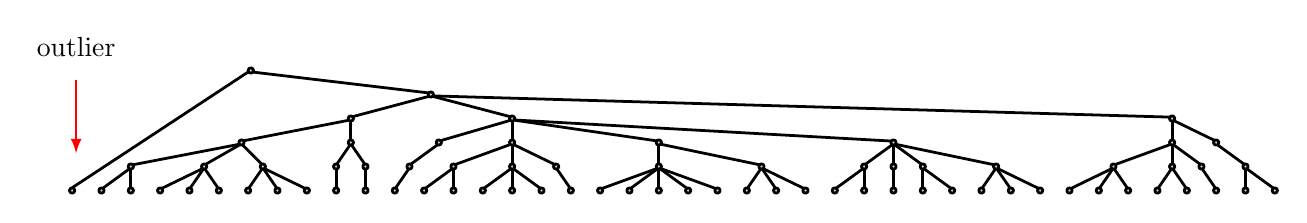
\begin{tikzpicture}[>=latex,line join=bevel,scale=0.48]
  \pgfsetlinewidth{1bp}
%%
\begin{scope}
  \pgfsetstrokecolor{black}
  \definecolor{strokecol}{rgb}{1.0,1.0,1.0};
  \pgfsetstrokecolor{strokecol}
  \definecolor{fillcol}{rgb}{1.0,1.0,1.0};
  \pgfsetfillcolor{fillcol}
  \filldraw (0bp,0bp) -- (0bp,94bp) -- (906bp,94bp) -- (906bp,0bp) -- cycle;
\end{scope}
\begin{scope}
  \pgfsetstrokecolor{black}
  \definecolor{strokecol}{rgb}{1.0,1.0,1.0};
  \pgfsetstrokecolor{strokecol}
  \definecolor{fillcol}{rgb}{1.0,1.0,1.0};
  \pgfsetfillcolor{fillcol}
  \filldraw (0bp,0bp) -- (0bp,94bp) -- (906bp,94bp) -- (906bp,0bp) -- cycle;
\end{scope}
\begin{scope}
  \pgfsetstrokecolor{black}
  \definecolor{strokecol}{rgb}{1.0,1.0,1.0};
  \pgfsetstrokecolor{strokecol}
  \definecolor{fillcol}{rgb}{1.0,1.0,1.0};
  \pgfsetfillcolor{fillcol}
  \filldraw (0bp,0bp) -- (0bp,94bp) -- (906bp,94bp) -- (906bp,0bp) -- cycle;
\end{scope}
\begin{scope}
  \pgfsetstrokecolor{black}
  \definecolor{strokecol}{rgb}{1.0,1.0,1.0};
  \pgfsetstrokecolor{strokecol}
  \definecolor{fillcol}{rgb}{1.0,1.0,1.0};
  \pgfsetfillcolor{fillcol}
  \filldraw (0bp,0bp) -- (0bp,94bp) -- (906bp,94bp) -- (906bp,0bp) -- cycle;
\end{scope}
\begin{scope}
  \pgfsetstrokecolor{black}
  \definecolor{strokecol}{rgb}{1.0,1.0,1.0};
  \pgfsetstrokecolor{strokecol}
  \definecolor{fillcol}{rgb}{1.0,1.0,1.0};
  \pgfsetfillcolor{fillcol}
  \filldraw (0bp,0bp) -- (0bp,94bp) -- (906bp,94bp) -- (906bp,0bp) -- cycle;
\end{scope}
\begin{scope}
  \pgfsetstrokecolor{black}
  \definecolor{strokecol}{rgb}{1.0,1.0,1.0};
  \pgfsetstrokecolor{strokecol}
  \definecolor{fillcol}{rgb}{1.0,1.0,1.0};
  \pgfsetfillcolor{fillcol}
  \filldraw (0bp,0bp) -- (0bp,94bp) -- (906bp,94bp) -- (906bp,0bp) -- cycle;
\end{scope}
\begin{scope}
  \pgfsetstrokecolor{black}
  \definecolor{strokecol}{rgb}{1.0,1.0,1.0};
  \pgfsetstrokecolor{strokecol}
  \definecolor{fillcol}{rgb}{1.0,1.0,1.0};
  \pgfsetfillcolor{fillcol}
  \filldraw (0bp,0bp) -- (0bp,94bp) -- (906bp,94bp) -- (906bp,0bp) -- cycle;
\end{scope}
\begin{scope}
  \pgfsetstrokecolor{black}
  \definecolor{strokecol}{rgb}{1.0,1.0,1.0};
  \pgfsetstrokecolor{strokecol}
  \definecolor{fillcol}{rgb}{1.0,1.0,1.0};
  \pgfsetfillcolor{fillcol}
  \filldraw (0bp,0bp) -- (0bp,94bp) -- (906bp,94bp) -- (906bp,0bp) -- cycle;
\end{scope}
\begin{scope}
  \pgfsetstrokecolor{black}
  \definecolor{strokecol}{rgb}{1.0,1.0,1.0};
  \pgfsetstrokecolor{strokecol}
  \definecolor{fillcol}{rgb}{1.0,1.0,1.0};
  \pgfsetfillcolor{fillcol}
  \filldraw (0bp,0bp) -- (0bp,94bp) -- (906bp,94bp) -- (906bp,0bp) -- cycle;
\end{scope}
\begin{scope}
  \pgfsetstrokecolor{black}
  \definecolor{strokecol}{rgb}{1.0,1.0,1.0};
  \pgfsetstrokecolor{strokecol}
  \definecolor{fillcol}{rgb}{1.0,1.0,1.0};
  \pgfsetfillcolor{fillcol}
  \filldraw (0bp,0bp) -- (0bp,94bp) -- (906bp,94bp) -- (906bp,0bp) -- cycle;
\end{scope}
\begin{scope}
  \pgfsetstrokecolor{black}
  \definecolor{strokecol}{rgb}{1.0,1.0,1.0};
  \pgfsetstrokecolor{strokecol}
  \definecolor{fillcol}{rgb}{1.0,1.0,1.0};
  \pgfsetfillcolor{fillcol}
  \filldraw (0bp,0bp) -- (0bp,94bp) -- (906bp,94bp) -- (906bp,0bp) -- cycle;
\end{scope}
\begin{scope}
  \pgfsetstrokecolor{black}
  \definecolor{strokecol}{rgb}{1.0,1.0,1.0};
  \pgfsetstrokecolor{strokecol}
  \definecolor{fillcol}{rgb}{1.0,1.0,1.0};
  \pgfsetfillcolor{fillcol}
  \filldraw (0bp,0bp) -- (0bp,94bp) -- (906bp,94bp) -- (906bp,0bp) -- cycle;
\end{scope}
\begin{scope}
  \pgfsetstrokecolor{black}
  \definecolor{strokecol}{rgb}{1.0,1.0,1.0};
  \pgfsetstrokecolor{strokecol}
  \definecolor{fillcol}{rgb}{1.0,1.0,1.0};
  \pgfsetfillcolor{fillcol}
  \filldraw (0bp,0bp) -- (0bp,94bp) -- (906bp,94bp) -- (906bp,0bp) -- cycle;
\end{scope}
\begin{scope}
  \pgfsetstrokecolor{black}
  \definecolor{strokecol}{rgb}{1.0,1.0,1.0};
  \pgfsetstrokecolor{strokecol}
  \definecolor{fillcol}{rgb}{1.0,1.0,1.0};
  \pgfsetfillcolor{fillcol}
  \filldraw (0bp,0bp) -- (0bp,94bp) -- (906bp,94bp) -- (906bp,0bp) -- cycle;
\end{scope}
\begin{scope}
  \pgfsetstrokecolor{black}
  \definecolor{strokecol}{rgb}{1.0,1.0,1.0};
  \pgfsetstrokecolor{strokecol}
  \definecolor{fillcol}{rgb}{1.0,1.0,1.0};
  \pgfsetfillcolor{fillcol}
  \filldraw (0bp,0bp) -- (0bp,94bp) -- (906bp,94bp) -- (906bp,0bp) -- cycle;
\end{scope}
\begin{scope}
  \pgfsetstrokecolor{black}
  \definecolor{strokecol}{rgb}{1.0,1.0,1.0};
  \pgfsetstrokecolor{strokecol}
  \definecolor{fillcol}{rgb}{1.0,1.0,1.0};
  \pgfsetfillcolor{fillcol}
  \filldraw (0bp,0bp) -- (0bp,94bp) -- (906bp,94bp) -- (906bp,0bp) -- cycle;
\end{scope}
\begin{scope}
  \pgfsetstrokecolor{black}
  \definecolor{strokecol}{rgb}{1.0,1.0,1.0};
  \pgfsetstrokecolor{strokecol}
  \definecolor{fillcol}{rgb}{1.0,1.0,1.0};
  \pgfsetfillcolor{fillcol}
  \filldraw (0bp,0bp) -- (0bp,94bp) -- (906bp,94bp) -- (906bp,0bp) -- cycle;
\end{scope}
\begin{scope}
  \pgfsetstrokecolor{black}
  \definecolor{strokecol}{rgb}{1.0,1.0,1.0};
  \pgfsetstrokecolor{strokecol}
  \definecolor{fillcol}{rgb}{1.0,1.0,1.0};
  \pgfsetfillcolor{fillcol}
  \filldraw (0bp,0bp) -- (0bp,94bp) -- (906bp,94bp) -- (906bp,0bp) -- cycle;
\end{scope}
\begin{scope}
  \pgfsetstrokecolor{black}
  \definecolor{strokecol}{rgb}{1.0,1.0,1.0};
  \pgfsetstrokecolor{strokecol}
  \definecolor{fillcol}{rgb}{1.0,1.0,1.0};
  \pgfsetfillcolor{fillcol}
  \filldraw (0bp,0bp) -- (0bp,94bp) -- (906bp,94bp) -- (906bp,0bp) -- cycle;
\end{scope}
\begin{scope}
  \pgfsetstrokecolor{black}
  \definecolor{strokecol}{rgb}{1.0,1.0,1.0};
  \pgfsetstrokecolor{strokecol}
  \definecolor{fillcol}{rgb}{1.0,1.0,1.0};
  \pgfsetfillcolor{fillcol}
  \filldraw (0bp,0bp) -- (0bp,94bp) -- (906bp,94bp) -- (906bp,0bp) -- cycle;
\end{scope}
\begin{scope}
  \pgfsetstrokecolor{black}
  \definecolor{strokecol}{rgb}{1.0,1.0,1.0};
  \pgfsetstrokecolor{strokecol}
  \definecolor{fillcol}{rgb}{1.0,1.0,1.0};
  \pgfsetfillcolor{fillcol}
  \filldraw (0bp,0bp) -- (0bp,94bp) -- (906bp,94bp) -- (906bp,0bp) -- cycle;
\end{scope}
\begin{scope}
  \pgfsetstrokecolor{black}
  \definecolor{strokecol}{rgb}{1.0,1.0,1.0};
  \pgfsetstrokecolor{strokecol}
  \definecolor{fillcol}{rgb}{1.0,1.0,1.0};
  \pgfsetfillcolor{fillcol}
  \filldraw (0bp,0bp) -- (0bp,94bp) -- (906bp,94bp) -- (906bp,0bp) -- cycle;
\end{scope}
\begin{scope}
  \pgfsetstrokecolor{black}
  \definecolor{strokecol}{rgb}{1.0,1.0,1.0};
  \pgfsetstrokecolor{strokecol}
  \definecolor{fillcol}{rgb}{1.0,1.0,1.0};
  \pgfsetfillcolor{fillcol}
  \filldraw (0bp,0bp) -- (0bp,94bp) -- (906bp,94bp) -- (906bp,0bp) -- cycle;
\end{scope}
\begin{scope}
  \pgfsetstrokecolor{black}
  \definecolor{strokecol}{rgb}{1.0,1.0,1.0};
  \pgfsetstrokecolor{strokecol}
  \definecolor{fillcol}{rgb}{1.0,1.0,1.0};
  \pgfsetfillcolor{fillcol}
  \filldraw (0bp,0bp) -- (0bp,94bp) -- (906bp,94bp) -- (906bp,0bp) -- cycle;
\end{scope}
\begin{scope}
  \pgfsetstrokecolor{black}
  \definecolor{strokecol}{rgb}{1.0,1.0,1.0};
  \pgfsetstrokecolor{strokecol}
  \definecolor{fillcol}{rgb}{1.0,1.0,1.0};
  \pgfsetfillcolor{fillcol}
  \filldraw (0bp,0bp) -- (0bp,94bp) -- (906bp,94bp) -- (906bp,0bp) -- cycle;
\end{scope}
\begin{scope}
  \pgfsetstrokecolor{black}
  \definecolor{strokecol}{rgb}{1.0,1.0,1.0};
  \pgfsetstrokecolor{strokecol}
  \definecolor{fillcol}{rgb}{1.0,1.0,1.0};
  \pgfsetfillcolor{fillcol}
  \filldraw (0bp,0bp) -- (0bp,94bp) -- (906bp,94bp) -- (906bp,0bp) -- cycle;
\end{scope}
\begin{scope}
  \pgfsetstrokecolor{black}
  \definecolor{strokecol}{rgb}{1.0,1.0,1.0};
  \pgfsetstrokecolor{strokecol}
  \definecolor{fillcol}{rgb}{1.0,1.0,1.0};
  \pgfsetfillcolor{fillcol}
  \filldraw (0bp,0bp) -- (0bp,94bp) -- (906bp,94bp) -- (906bp,0bp) -- cycle;
\end{scope}
\begin{scope}
  \pgfsetstrokecolor{black}
  \definecolor{strokecol}{rgb}{1.0,1.0,1.0};
  \pgfsetstrokecolor{strokecol}
  \definecolor{fillcol}{rgb}{1.0,1.0,1.0};
  \pgfsetfillcolor{fillcol}
  \filldraw (0bp,0bp) -- (0bp,94bp) -- (906bp,94bp) -- (906bp,0bp) -- cycle;
\end{scope}
  \pgfsetcolor{black}
  % Edge: c12 -> c30
  \draw [-] (827bp,35.95bp) -- (827bp,22.075bp);
  % Edge: c8 -> c19
  \draw [-] (275.82bp,36.14bp) -- (256.08bp,21.788bp);
  % Edge: c23 -> c54
  \draw [-] (443.46bp,18.468bp) -- (484.49bp,3.5508bp);
  % Edge: c28 -> c65
  \draw [-] (696.42bp,18.312bp) -- (726.62bp,3.6671bp);
  % Edge: c6 -> c16
  \draw [-] (130.05bp,35.95bp) -- (143.93bp,22.075bp);
  % Edge: c18 -> c42
  \draw [-] (222bp,17.95bp) -- (222bp,4.0746bp);
  % Edge: c2 -> c4
  \draw [-] (272.51bp,72.604bp) -- (330.32bp,57.44bp);
  % Edge: c27 -> c61
  \draw [-] (640bp,17.95bp) -- (640bp,4.0746bp);
  % Edge: c4 -> c8
  \draw [-] (330.17bp,54.468bp) -- (278.46bp,39.426bp);
  % Edge: c7 -> c17
  \draw [-] (210.28bp,35.95bp) -- (200.74bp,22.075bp);
  % Edge: c16 -> c38
  \draw [-] (144.28bp,17.95bp) -- (134.74bp,4.0746bp);
  % Edge: c10 -> c24
  \draw [-] (443.61bp,36.666bp) -- (517.4bp,21.332bp);
  % Edge: c23 -> c50
  \draw [-] (440.54bp,18.468bp) -- (399.51bp,3.5508bp);
  % Edge: c4 -> c10
  \draw [-] (333.91bp,54.722bp) -- (440.37bp,39.237bp);
  % Edge: c29 -> c67
  \draw [-] (782.28bp,17.95bp) -- (772.74bp,4.0746bp);
  % Edge: c12 -> c29
  \draw [-] (825.54bp,36.468bp) -- (784.51bp,21.551bp);
  % Edge: c23 -> c51
  \draw [-] (440.82bp,18.14bp) -- (421.08bp,3.788bp);
  % Edge: c16 -> c40
  \draw [-] (146.42bp,18.312bp) -- (176.62bp,3.6671bp);
  % Edge: root -> c2
  \draw [-] (137.91bp,90.774bp) -- (269.34bp,75.196bp);
  % Edge: c12 -> c31
  \draw [-] (828.18bp,36.14bp) -- (847.92bp,21.788bp);
  % Edge: c17 -> c41
  \draw [-] (200bp,17.95bp) -- (200bp,4.0746bp);
  % Edge: c2 -> c5
  \draw [-] (273.01bp,72.942bp) -- (825.12bp,57.054bp);
  % Edge: c23 -> c52
  \draw [-] (442bp,17.95bp) -- (442bp,4.0746bp);
  % Edge: c4 -> c9
  \draw [-] (332bp,53.95bp) -- (332bp,40.075bp);
  % Edge: c9 -> c20
  \draw [-] (330.54bp,36.468bp) -- (289.51bp,21.551bp);
  % Edge: c27 -> c62
  \draw [-] (641.18bp,18.14bp) -- (660.92bp,3.788bp);
  % Edge: c16 -> c39
  \draw [-] (145.72bp,17.95bp) -- (155.26bp,4.0746bp);
  % Edge: c22 -> c49
  \draw [-] (365.72bp,17.95bp) -- (375.26bp,4.0746bp);
  % Edge: c4 -> c11
  \draw [-] (333.83bp,54.898bp) -- (616.05bp,39.109bp);
  % Edge: c23 -> c53
  \draw [-] (443.18bp,18.14bp) -- (462.92bp,3.788bp);
  % Edge: c20 -> c44
  \draw [-] (286.82bp,18.14bp) -- (267.08bp,3.788bp);
  % Edge: c32 -> c73
  \draw [-] (883.18bp,18.14bp) -- (902.92bp,3.788bp);
  % Edge: c11 -> c25
  \draw [-] (616.82bp,36.14bp) -- (597.08bp,21.788bp);
  % Edge: root -> c1
  \draw [-] (134.11bp,90.943bp) -- (2bp,4.0576bp);
  % Edge: c15 -> c37
  \draw [-] (101.72bp,17.95bp) -- (111.26bp,4.0746bp);
  % Edge: c21 -> c46
  \draw [-] (330.82bp,18.14bp) -- (311.08bp,3.788bp);
  % Edge: c7 -> c18
  \draw [-] (211.72bp,35.95bp) -- (221.26bp,22.075bp);
  % Edge: c25 -> c59
  \draw [-] (596bp,17.95bp) -- (596bp,4.0746bp);
  % Edge: c10 -> c23
  \draw [-] (442bp,35.95bp) -- (442bp,22.075bp);
  % Edge: c9 -> c21
  \draw [-] (332bp,35.95bp) -- (332bp,22.075bp);
  % Edge: c3 -> c7
  \draw [-] (211bp,53.95bp) -- (211bp,40.075bp);
  % Edge: c30 -> c70
  \draw [-] (827.72bp,17.95bp) -- (837.26bp,4.0746bp);
  % Edge: c28 -> c63
  \draw [-] (694.28bp,17.95bp) -- (684.74bp,4.0746bp);
  % Edge: c6 -> c14
  \draw [-] (127.27bp,36.666bp) -- (47.724bp,21.332bp);
  % Edge: c24 -> c57
  \draw [-] (520.42bp,18.312bp) -- (550.62bp,3.6671bp);
  % Edge: c20 -> c45
  \draw [-] (288bp,17.95bp) -- (288bp,4.0746bp);
  % Edge: c26 -> c60
  \draw [-] (618bp,17.95bp) -- (618bp,4.0746bp);
  % Edge: c14 -> c34
  \draw [-] (46bp,17.95bp) -- (46bp,4.0746bp);
  % Edge: c11 -> c26
  \draw [-] (618bp,35.95bp) -- (618bp,22.075bp);
  % Edge: c21 -> c48
  \draw [-] (333.18bp,18.14bp) -- (352.92bp,3.788bp);
  % Edge: c14 -> c33
  \draw [-] (44.817bp,18.14bp) -- (25.083bp,3.788bp);
  % Edge: c31 -> c71
  \draw [-] (849.72bp,17.95bp) -- (859.26bp,4.0746bp);
  % Edge: c5 -> c13
  \draw [-] (828.42bp,54.312bp) -- (858.62bp,39.667bp);
  % Edge: c13 -> c32
  \draw [-] (861.18bp,36.14bp) -- (880.92bp,21.788bp);
  % Edge: c25 -> c58
  \draw [-] (594.82bp,18.14bp) -- (575.08bp,3.788bp);
  % Edge: c15 -> c36
  \draw [-] (100.28bp,17.95bp) -- (90.739bp,4.0746bp);
  % Edge: c9 -> c22
  \draw [-] (333.42bp,36.312bp) -- (363.62bp,21.667bp);
  % Edge: c3 -> c6
  \draw [-] (209.29bp,54.666bp) -- (130.7bp,39.332bp);
  % Edge: c21 -> c47
  \draw [-] (332bp,17.95bp) -- (332bp,4.0746bp);
  % Edge: c30 -> c69
  \draw [-] (826.28bp,17.95bp) -- (816.74bp,4.0746bp);
  % Edge: c28 -> c64
  \draw [-] (695.72bp,17.95bp) -- (705.26bp,4.0746bp);
  % Edge: c6 -> c15
  \draw [-] (127.8bp,36.312bp) -- (102.17bp,21.667bp);
  % Edge: c2 -> c3
  \draw [-] (269.52bp,72.604bp) -- (212.65bp,57.44bp);
  % Edge: c19 -> c43
  \draw [-] (254.28bp,17.95bp) -- (244.74bp,4.0746bp);
  % Edge: c29 -> c66
  \draw [-] (781.58bp,18.312bp) -- (751.38bp,3.6671bp);
  % Edge: c11 -> c27
  \draw [-] (619.18bp,36.14bp) -- (638.92bp,21.788bp);
  % Edge: c24 -> c55
  \draw [-] (518.28bp,17.95bp) -- (508.74bp,4.0746bp);
  % Edge: c24 -> c56
  \draw [-] (519.72bp,17.95bp) -- (529.26bp,4.0746bp);
  % Edge: c11 -> c28
  \draw [-] (619.61bp,36.666bp) -- (693.4bp,21.332bp);
  % Edge: c32 -> c72
  \draw [-] (882bp,17.95bp) -- (882bp,4.0746bp);
  % Edge: c5 -> c12
  \draw [-] (827bp,53.95bp) -- (827bp,40.075bp);
  % Edge: c15 -> c35
  \draw [-] (99.582bp,18.312bp) -- (69.376bp,3.6671bp);
  % Edge: c29 -> c68
  \draw [-] (783.72bp,17.95bp) -- (793.26bp,4.0746bp);
  % Node: c10
\begin{scope}
  \definecolor{strokecol}{rgb}{0.0,0.0,0.0};
  \pgfsetstrokecolor{strokecol}
  \definecolor{fillcol}{rgb}{0.83,0.83,0.83};
  \pgfsetfillcolor{fillcol}
  \filldraw [opacity=1] (442bp,38bp) ellipse (2bp and 2bp);
\end{scope}
  % Node: c65
\begin{scope}
  \definecolor{strokecol}{rgb}{0.0,0.0,0.0};
  \pgfsetstrokecolor{strokecol}
  \definecolor{fillcol}{rgb}{0.83,0.83,0.83};
  \pgfsetfillcolor{fillcol}
  \filldraw [opacity=1] (728bp,2bp) ellipse (2bp and 2bp);
\end{scope}
  % Node: c69
\begin{scope}
  \definecolor{strokecol}{rgb}{0.0,0.0,0.0};
  \pgfsetstrokecolor{strokecol}
  \definecolor{fillcol}{rgb}{0.83,0.83,0.83};
  \pgfsetfillcolor{fillcol}
  \filldraw [opacity=1] (816bp,2bp) ellipse (2bp and 2bp);
\end{scope}
  % Node: c62
\begin{scope}
  \definecolor{strokecol}{rgb}{0.0,0.0,0.0};
  \pgfsetstrokecolor{strokecol}
  \definecolor{fillcol}{rgb}{0.83,0.83,0.83};
  \pgfsetfillcolor{fillcol}
  \filldraw [opacity=1] (662bp,2bp) ellipse (2bp and 2bp);
\end{scope}
  % Node: c63
\begin{scope}
  \definecolor{strokecol}{rgb}{0.0,0.0,0.0};
  \pgfsetstrokecolor{strokecol}
  \definecolor{fillcol}{rgb}{0.83,0.83,0.83};
  \pgfsetfillcolor{fillcol}
  \filldraw [opacity=1] (684bp,2bp) ellipse (2bp and 2bp);
\end{scope}
  % Node: c4
\begin{scope}
  \definecolor{strokecol}{rgb}{0.0,0.0,0.0};
  \pgfsetstrokecolor{strokecol}
  \definecolor{fillcol}{rgb}{0.83,0.83,0.83};
  \pgfsetfillcolor{fillcol}
  \filldraw [opacity=1] (332bp,56bp) ellipse (2bp and 2bp);
\end{scope}
  % Node: c2
\begin{scope}
  \definecolor{strokecol}{rgb}{0.0,0.0,0.0};
  \pgfsetstrokecolor{strokecol}
  \definecolor{fillcol}{rgb}{0.83,0.83,0.83};
  \pgfsetfillcolor{fillcol}
  \filldraw [opacity=1] (271bp,74bp) ellipse (2bp and 2bp);
\end{scope}
  % Node: c61
\begin{scope}
  \definecolor{strokecol}{rgb}{0.0,0.0,0.0};
  \pgfsetstrokecolor{strokecol}
  \definecolor{fillcol}{rgb}{0.83,0.83,0.83};
  \pgfsetfillcolor{fillcol}
  \filldraw [opacity=1] (640bp,2bp) ellipse (2bp and 2bp);
\end{scope}
  % Node: c57
\begin{scope}
  \definecolor{strokecol}{rgb}{0.0,0.0,0.0};
  \pgfsetstrokecolor{strokecol}
  \definecolor{fillcol}{rgb}{0.83,0.83,0.83};
  \pgfsetfillcolor{fillcol}
  \filldraw [opacity=1] (552bp,2bp) ellipse (2bp and 2bp);
\end{scope}
  % Node: c56
\begin{scope}
  \definecolor{strokecol}{rgb}{0.0,0.0,0.0};
  \pgfsetstrokecolor{strokecol}
  \definecolor{fillcol}{rgb}{0.83,0.83,0.83};
  \pgfsetfillcolor{fillcol}
  \filldraw [opacity=1] (530bp,2bp) ellipse (2bp and 2bp);
\end{scope}
  % Node: c55
\begin{scope}
  \definecolor{strokecol}{rgb}{0.0,0.0,0.0};
  \pgfsetstrokecolor{strokecol}
  \definecolor{fillcol}{rgb}{0.83,0.83,0.83};
  \pgfsetfillcolor{fillcol}
  \filldraw [opacity=1] (508bp,2bp) ellipse (2bp and 2bp);
\end{scope}
  % Node: c54
\begin{scope}
  \definecolor{strokecol}{rgb}{0.0,0.0,0.0};
  \pgfsetstrokecolor{strokecol}
  \definecolor{fillcol}{rgb}{0.83,0.83,0.83};
  \pgfsetfillcolor{fillcol}
  \filldraw [opacity=1] (486bp,2bp) ellipse (2bp and 2bp);
\end{scope}
  % Node: c53
\begin{scope}
  \definecolor{strokecol}{rgb}{0.0,0.0,0.0};
  \pgfsetstrokecolor{strokecol}
  \definecolor{fillcol}{rgb}{0.83,0.83,0.83};
  \pgfsetfillcolor{fillcol}
  \filldraw [opacity=1] (464bp,2bp) ellipse (2bp and 2bp);
\end{scope}
  % Node: c52
\begin{scope}
  \definecolor{strokecol}{rgb}{0.0,0.0,0.0};
  \pgfsetstrokecolor{strokecol}
  \definecolor{fillcol}{rgb}{0.83,0.83,0.83};
  \pgfsetfillcolor{fillcol}
  \filldraw [opacity=1] (442bp,2bp) ellipse (2bp and 2bp);
\end{scope}
  % Node: c51
\begin{scope}
  \definecolor{strokecol}{rgb}{0.0,0.0,0.0};
  \pgfsetstrokecolor{strokecol}
  \definecolor{fillcol}{rgb}{0.83,0.83,0.83};
  \pgfsetfillcolor{fillcol}
  \filldraw [opacity=1] (420bp,2bp) ellipse (2bp and 2bp);
\end{scope}
  % Node: c50
\begin{scope}
  \definecolor{strokecol}{rgb}{0.0,0.0,0.0};
  \pgfsetstrokecolor{strokecol}
  \definecolor{fillcol}{rgb}{0.83,0.83,0.83};
  \pgfsetfillcolor{fillcol}
  \filldraw [opacity=1] (398bp,2bp) ellipse (2bp and 2bp);
\end{scope}
  % Node: c71
\begin{scope}
  \definecolor{strokecol}{rgb}{0.0,0.0,0.0};
  \pgfsetstrokecolor{strokecol}
  \definecolor{fillcol}{rgb}{0.83,0.83,0.83};
  \pgfsetfillcolor{fillcol}
  \filldraw [opacity=1] (860bp,2bp) ellipse (2bp and 2bp);
\end{scope}
  % Node: c70
\begin{scope}
  \definecolor{strokecol}{rgb}{0.0,0.0,0.0};
  \pgfsetstrokecolor{strokecol}
  \definecolor{fillcol}{rgb}{0.83,0.83,0.83};
  \pgfsetfillcolor{fillcol}
  \filldraw [opacity=1] (838bp,2bp) ellipse (2bp and 2bp);
\end{scope}
  % Node: c73
\begin{scope}
  \definecolor{strokecol}{rgb}{0.0,0.0,0.0};
  \pgfsetstrokecolor{strokecol}
  \definecolor{fillcol}{rgb}{0.83,0.83,0.83};
  \pgfsetfillcolor{fillcol}
  \filldraw [opacity=1] (904bp,2bp) ellipse (2bp and 2bp);
\end{scope}
  % Node: c72
\begin{scope}
  \definecolor{strokecol}{rgb}{0.0,0.0,0.0};
  \pgfsetstrokecolor{strokecol}
  \definecolor{fillcol}{rgb}{0.83,0.83,0.83};
  \pgfsetfillcolor{fillcol}
  \filldraw [opacity=1] (882bp,2bp) ellipse (2bp and 2bp);
\end{scope}
  % Node: c59
\begin{scope}
  \definecolor{strokecol}{rgb}{0.0,0.0,0.0};
  \pgfsetstrokecolor{strokecol}
  \definecolor{fillcol}{rgb}{0.83,0.83,0.83};
  \pgfsetfillcolor{fillcol}
  \filldraw [opacity=1] (596bp,2bp) ellipse (2bp and 2bp);
\end{scope}
  % Node: c58
\begin{scope}
  \definecolor{strokecol}{rgb}{0.0,0.0,0.0};
  \pgfsetstrokecolor{strokecol}
  \definecolor{fillcol}{rgb}{0.83,0.83,0.83};
  \pgfsetfillcolor{fillcol}
  \filldraw [opacity=1] (574bp,2bp) ellipse (2bp and 2bp);
\end{scope}
  % Node: c19
\begin{scope}
  \definecolor{strokecol}{rgb}{0.0,0.0,0.0};
  \pgfsetstrokecolor{strokecol}
  \definecolor{fillcol}{rgb}{0.83,0.83,0.83};
  \pgfsetfillcolor{fillcol}
  \filldraw [opacity=1] (255bp,20bp) ellipse (2bp and 2bp);
\end{scope}
  % Node: c18
\begin{scope}
  \definecolor{strokecol}{rgb}{0.0,0.0,0.0};
  \pgfsetstrokecolor{strokecol}
  \definecolor{fillcol}{rgb}{0.83,0.83,0.83};
  \pgfsetfillcolor{fillcol}
  \filldraw [opacity=1] (222bp,20bp) ellipse (2bp and 2bp);
\end{scope}
  % Node: c39
\begin{scope}
  \definecolor{strokecol}{rgb}{0.0,0.0,0.0};
  \pgfsetstrokecolor{strokecol}
  \definecolor{fillcol}{rgb}{0.83,0.83,0.83};
  \pgfsetfillcolor{fillcol}
  \filldraw [opacity=1] (156bp,2bp) ellipse (2bp and 2bp);
\end{scope}
  % Node: c38
\begin{scope}
  \definecolor{strokecol}{rgb}{0.0,0.0,0.0};
  \pgfsetstrokecolor{strokecol}
  \definecolor{fillcol}{rgb}{0.83,0.83,0.83};
  \pgfsetfillcolor{fillcol}
  \filldraw [opacity=1] (134bp,2bp) ellipse (2bp and 2bp);
\end{scope}
  % Node: c35
\begin{scope}
  \definecolor{strokecol}{rgb}{0.0,0.0,0.0};
  \pgfsetstrokecolor{strokecol}
  \definecolor{fillcol}{rgb}{0.83,0.83,0.83};
  \pgfsetfillcolor{fillcol}
  \filldraw [opacity=1] (68bp,2bp) ellipse (2bp and 2bp);
\end{scope}
  % Node: c34
\begin{scope}
  \definecolor{strokecol}{rgb}{0.0,0.0,0.0};
  \pgfsetstrokecolor{strokecol}
  \definecolor{fillcol}{rgb}{0.83,0.83,0.83};
  \pgfsetfillcolor{fillcol}
  \filldraw [opacity=1] (46bp,2bp) ellipse (2bp and 2bp);
\end{scope}
  % Node: c37
\begin{scope}
  \definecolor{strokecol}{rgb}{0.0,0.0,0.0};
  \pgfsetstrokecolor{strokecol}
  \definecolor{fillcol}{rgb}{0.83,0.83,0.83};
  \pgfsetfillcolor{fillcol}
  \filldraw [opacity=1] (112bp,2bp) ellipse (2bp and 2bp);
\end{scope}
  % Node: c36
\begin{scope}
  \definecolor{strokecol}{rgb}{0.0,0.0,0.0};
  \pgfsetstrokecolor{strokecol}
  \definecolor{fillcol}{rgb}{0.83,0.83,0.83};
  \pgfsetfillcolor{fillcol}
  \filldraw [opacity=1] (90bp,2bp) ellipse (2bp and 2bp);
\end{scope}
  % Node: c31
\begin{scope}
  \definecolor{strokecol}{rgb}{0.0,0.0,0.0};
  \pgfsetstrokecolor{strokecol}
  \definecolor{fillcol}{rgb}{0.83,0.83,0.83};
  \pgfsetfillcolor{fillcol}
  \filldraw [opacity=1] (849bp,20bp) ellipse (2bp and 2bp);
\end{scope}
  % Node: c30
\begin{scope}
  \definecolor{strokecol}{rgb}{0.0,0.0,0.0};
  \pgfsetstrokecolor{strokecol}
  \definecolor{fillcol}{rgb}{0.83,0.83,0.83};
  \pgfsetfillcolor{fillcol}
  \filldraw [opacity=1] (827bp,20bp) ellipse (2bp and 2bp);
\end{scope}
  % Node: c33
\begin{scope}
  \definecolor{strokecol}{rgb}{0.0,0.0,0.0};
  \pgfsetstrokecolor{strokecol}
  \definecolor{fillcol}{rgb}{0.83,0.83,0.83};
  \pgfsetfillcolor{fillcol}
  \filldraw [opacity=1] (24bp,2bp) ellipse (2bp and 2bp);
\end{scope}
  % Node: c32
\begin{scope}
  \definecolor{strokecol}{rgb}{0.0,0.0,0.0};
  \pgfsetstrokecolor{strokecol}
  \definecolor{fillcol}{rgb}{0.83,0.83,0.83};
  \pgfsetfillcolor{fillcol}
  \filldraw [opacity=1] (882bp,20bp) ellipse (2bp and 2bp);
\end{scope}
  % Node: c44
\begin{scope}
  \definecolor{strokecol}{rgb}{0.0,0.0,0.0};
  \pgfsetstrokecolor{strokecol}
  \definecolor{fillcol}{rgb}{0.83,0.83,0.83};
  \pgfsetfillcolor{fillcol}
  \filldraw [opacity=1] (266bp,2bp) ellipse (2bp and 2bp);
\end{scope}
  % Node: c68
\begin{scope}
  \definecolor{strokecol}{rgb}{0.0,0.0,0.0};
  \pgfsetstrokecolor{strokecol}
  \definecolor{fillcol}{rgb}{0.83,0.83,0.83};
  \pgfsetfillcolor{fillcol}
  \filldraw [opacity=1] (794bp,2bp) ellipse (2bp and 2bp);
\end{scope}
  % Node: c11
\begin{scope}
  \definecolor{strokecol}{rgb}{0.0,0.0,0.0};
  \pgfsetstrokecolor{strokecol}
  \definecolor{fillcol}{rgb}{0.83,0.83,0.83};
  \pgfsetfillcolor{fillcol}
  \filldraw [opacity=1] (618bp,38bp) ellipse (2bp and 2bp);
\end{scope}
  % Node: c42
\begin{scope}
  \definecolor{strokecol}{rgb}{0.0,0.0,0.0};
  \pgfsetstrokecolor{strokecol}
  \definecolor{fillcol}{rgb}{0.83,0.83,0.83};
  \pgfsetfillcolor{fillcol}
  \filldraw [opacity=1] (222bp,2bp) ellipse (2bp and 2bp);
\end{scope}
  % Node: c45
\begin{scope}
  \definecolor{strokecol}{rgb}{0.0,0.0,0.0};
  \pgfsetstrokecolor{strokecol}
  \definecolor{fillcol}{rgb}{0.83,0.83,0.83};
  \pgfsetfillcolor{fillcol}
  \filldraw [opacity=1] (288bp,2bp) ellipse (2bp and 2bp);
\end{scope}
  % Node: c46
\begin{scope}
  \definecolor{strokecol}{rgb}{0.0,0.0,0.0};
  \pgfsetstrokecolor{strokecol}
  \definecolor{fillcol}{rgb}{0.83,0.83,0.83};
  \pgfsetfillcolor{fillcol}
  \filldraw [opacity=1] (310bp,2bp) ellipse (2bp and 2bp);
\end{scope}
  % Node: c13
\begin{scope}
  \definecolor{strokecol}{rgb}{0.0,0.0,0.0};
  \pgfsetstrokecolor{strokecol}
  \definecolor{fillcol}{rgb}{0.83,0.83,0.83};
  \pgfsetfillcolor{fillcol}
  \filldraw [opacity=1] (860bp,38bp) ellipse (2bp and 2bp);
\end{scope}
  % Node: c9
\begin{scope}
  \definecolor{strokecol}{rgb}{0.0,0.0,0.0};
  \pgfsetstrokecolor{strokecol}
  \definecolor{fillcol}{rgb}{0.83,0.83,0.83};
  \pgfsetfillcolor{fillcol}
  \filldraw [opacity=1] (332bp,38bp) ellipse (2bp and 2bp);
\end{scope}
  % Node: c47
\begin{scope}
  \definecolor{strokecol}{rgb}{0.0,0.0,0.0};
  \pgfsetstrokecolor{strokecol}
  \definecolor{fillcol}{rgb}{0.83,0.83,0.83};
  \pgfsetfillcolor{fillcol}
  \filldraw [opacity=1] (332bp,2bp) ellipse (2bp and 2bp);
\end{scope}
  % Node: c12
\begin{scope}
  \definecolor{strokecol}{rgb}{0.0,0.0,0.0};
  \pgfsetstrokecolor{strokecol}
  \definecolor{fillcol}{rgb}{0.83,0.83,0.83};
  \pgfsetfillcolor{fillcol}
  \filldraw [opacity=1] (827bp,38bp) ellipse (2bp and 2bp);
\end{scope}
  % Node: c3
\begin{scope}
  \definecolor{strokecol}{rgb}{0.0,0.0,0.0};
  \pgfsetstrokecolor{strokecol}
  \definecolor{fillcol}{rgb}{0.83,0.83,0.83};
  \pgfsetfillcolor{fillcol}
  \filldraw [opacity=1] (211bp,56bp) ellipse (2bp and 2bp);
\end{scope}
  % Node: c40
\begin{scope}
  \definecolor{strokecol}{rgb}{0.0,0.0,0.0};
  \pgfsetstrokecolor{strokecol}
  \definecolor{fillcol}{rgb}{0.83,0.83,0.83};
  \pgfsetfillcolor{fillcol}
  \filldraw [opacity=1] (178bp,2bp) ellipse (2bp and 2bp);
\end{scope}
  % Node: c1
\begin{scope}
  \definecolor{strokecol}{rgb}{0.0,0.0,0.0};
  \pgfsetstrokecolor{strokecol}
  \definecolor{fillcol}{rgb}{0.83,0.83,0.83};
  \pgfsetfillcolor{fillcol}
  \filldraw [opacity=1] (2bp,2bp) ellipse (2bp and 2bp);
\end{scope}
  % Node: c7
\begin{scope}
  \definecolor{strokecol}{rgb}{0.0,0.0,0.0};
  \pgfsetstrokecolor{strokecol}
  \definecolor{fillcol}{rgb}{0.83,0.83,0.83};
  \pgfsetfillcolor{fillcol}
  \filldraw [opacity=1] (211bp,38bp) ellipse (2bp and 2bp);
\end{scope}
  % Node: c6
\begin{scope}
  \definecolor{strokecol}{rgb}{0.0,0.0,0.0};
  \pgfsetstrokecolor{strokecol}
  \definecolor{fillcol}{rgb}{0.83,0.83,0.83};
  \pgfsetfillcolor{fillcol}
  \filldraw [opacity=1] (129bp,38bp) ellipse (2bp and 2bp);
\end{scope}
  % Node: c5
\begin{scope}
  \definecolor{strokecol}{rgb}{0.0,0.0,0.0};
  \pgfsetstrokecolor{strokecol}
  \definecolor{fillcol}{rgb}{0.83,0.83,0.83};
  \pgfsetfillcolor{fillcol}
  \filldraw [opacity=1] (827bp,56bp) ellipse (2bp and 2bp);
\end{scope}
  % Node: c41
\begin{scope}
  \definecolor{strokecol}{rgb}{0.0,0.0,0.0};
  \pgfsetstrokecolor{strokecol}
  \definecolor{fillcol}{rgb}{0.83,0.83,0.83};
  \pgfsetfillcolor{fillcol}
  \filldraw [opacity=1] (200bp,2bp) ellipse (2bp and 2bp);
\end{scope}
  % Node: c22
\begin{scope}
  \definecolor{strokecol}{rgb}{0.0,0.0,0.0};
  \pgfsetstrokecolor{strokecol}
  \definecolor{fillcol}{rgb}{0.83,0.83,0.83};
  \pgfsetfillcolor{fillcol}
  \filldraw [opacity=1] (365bp,20bp) ellipse (2bp and 2bp);
\end{scope}
  % Node: c23
\begin{scope}
  \definecolor{strokecol}{rgb}{0.0,0.0,0.0};
  \pgfsetstrokecolor{strokecol}
  \definecolor{fillcol}{rgb}{0.83,0.83,0.83};
  \pgfsetfillcolor{fillcol}
  \filldraw [opacity=1] (442bp,20bp) ellipse (2bp and 2bp);
\end{scope}
  % Node: c20
\begin{scope}
  \definecolor{strokecol}{rgb}{0.0,0.0,0.0};
  \pgfsetstrokecolor{strokecol}
  \definecolor{fillcol}{rgb}{0.83,0.83,0.83};
  \pgfsetfillcolor{fillcol}
  \filldraw [opacity=1] (288bp,20bp) ellipse (2bp and 2bp);
\end{scope}
  % Node: c21
\begin{scope}
  \definecolor{strokecol}{rgb}{0.0,0.0,0.0};
  \pgfsetstrokecolor{strokecol}
  \definecolor{fillcol}{rgb}{0.83,0.83,0.83};
  \pgfsetfillcolor{fillcol}
  \filldraw [opacity=1] (332bp,20bp) ellipse (2bp and 2bp);
\end{scope}
  % Node: c26
\begin{scope}
  \definecolor{strokecol}{rgb}{0.0,0.0,0.0};
  \pgfsetstrokecolor{strokecol}
  \definecolor{fillcol}{rgb}{0.83,0.83,0.83};
  \pgfsetfillcolor{fillcol}
  \filldraw [opacity=1] (618bp,20bp) ellipse (2bp and 2bp);
\end{scope}
  % Node: c27
\begin{scope}
  \definecolor{strokecol}{rgb}{0.0,0.0,0.0};
  \pgfsetstrokecolor{strokecol}
  \definecolor{fillcol}{rgb}{0.83,0.83,0.83};
  \pgfsetfillcolor{fillcol}
  \filldraw [opacity=1] (640bp,20bp) ellipse (2bp and 2bp);
\end{scope}
  % Node: c24
\begin{scope}
  \definecolor{strokecol}{rgb}{0.0,0.0,0.0};
  \pgfsetstrokecolor{strokecol}
  \definecolor{fillcol}{rgb}{0.83,0.83,0.83};
  \pgfsetfillcolor{fillcol}
  \filldraw [opacity=1] (519bp,20bp) ellipse (2bp and 2bp);
\end{scope}
  % Node: c25
\begin{scope}
  \definecolor{strokecol}{rgb}{0.0,0.0,0.0};
  \pgfsetstrokecolor{strokecol}
  \definecolor{fillcol}{rgb}{0.83,0.83,0.83};
  \pgfsetfillcolor{fillcol}
  \filldraw [opacity=1] (596bp,20bp) ellipse (2bp and 2bp);
\end{scope}
  % Node: c66
\begin{scope}
  \definecolor{strokecol}{rgb}{0.0,0.0,0.0};
  \pgfsetstrokecolor{strokecol}
  \definecolor{fillcol}{rgb}{0.83,0.83,0.83};
  \pgfsetfillcolor{fillcol}
  \filldraw [opacity=1] (750bp,2bp) ellipse (2bp and 2bp);
\end{scope}
  % Node: c17
\begin{scope}
  \definecolor{strokecol}{rgb}{0.0,0.0,0.0};
  \pgfsetstrokecolor{strokecol}
  \definecolor{fillcol}{rgb}{0.83,0.83,0.83};
  \pgfsetfillcolor{fillcol}
  \filldraw [opacity=1] (200bp,20bp) ellipse (2bp and 2bp);
\end{scope}
  % Node: c28
\begin{scope}
  \definecolor{strokecol}{rgb}{0.0,0.0,0.0};
  \pgfsetstrokecolor{strokecol}
  \definecolor{fillcol}{rgb}{0.83,0.83,0.83};
  \pgfsetfillcolor{fillcol}
  \filldraw [opacity=1] (695bp,20bp) ellipse (2bp and 2bp);
\end{scope}
  % Node: c29
\begin{scope}
  \definecolor{strokecol}{rgb}{0.0,0.0,0.0};
  \pgfsetstrokecolor{strokecol}
  \definecolor{fillcol}{rgb}{0.83,0.83,0.83};
  \pgfsetfillcolor{fillcol}
  \filldraw [opacity=1] (783bp,20bp) ellipse (2bp and 2bp);
\end{scope}
  % Node: c48
\begin{scope}
  \definecolor{strokecol}{rgb}{0.0,0.0,0.0};
  \pgfsetstrokecolor{strokecol}
  \definecolor{fillcol}{rgb}{0.83,0.83,0.83};
  \pgfsetfillcolor{fillcol}
  \filldraw [opacity=1] (354bp,2bp) ellipse (2bp and 2bp);
\end{scope}
  % Node: c49
\begin{scope}
  \definecolor{strokecol}{rgb}{0.0,0.0,0.0};
  \pgfsetstrokecolor{strokecol}
  \definecolor{fillcol}{rgb}{0.83,0.83,0.83};
  \pgfsetfillcolor{fillcol}
  \filldraw [opacity=1] (376bp,2bp) ellipse (2bp and 2bp);
\end{scope}
  % Node: c60
\begin{scope}
  \definecolor{strokecol}{rgb}{0.0,0.0,0.0};
  \pgfsetstrokecolor{strokecol}
  \definecolor{fillcol}{rgb}{0.83,0.83,0.83};
  \pgfsetfillcolor{fillcol}
  \filldraw [opacity=1] (618bp,2bp) ellipse (2bp and 2bp);
\end{scope}
  % Node: c16
\begin{scope}
  \definecolor{strokecol}{rgb}{0.0,0.0,0.0};
  \pgfsetstrokecolor{strokecol}
  \definecolor{fillcol}{rgb}{0.83,0.83,0.83};
  \pgfsetfillcolor{fillcol}
  \filldraw [opacity=1] (145bp,20bp) ellipse (2bp and 2bp);
\end{scope}
  % Node: c8
\begin{scope}
  \definecolor{strokecol}{rgb}{0.0,0.0,0.0};
  \pgfsetstrokecolor{strokecol}
  \definecolor{fillcol}{rgb}{0.83,0.83,0.83};
  \pgfsetfillcolor{fillcol}
  \filldraw [opacity=1] (277bp,38bp) ellipse (2bp and 2bp);
\end{scope}
  % Node: c15
\begin{scope}
  \definecolor{strokecol}{rgb}{0.0,0.0,0.0};
  \pgfsetstrokecolor{strokecol}
  \definecolor{fillcol}{rgb}{0.83,0.83,0.83};
  \pgfsetfillcolor{fillcol}
  \filldraw [opacity=1] (101bp,20bp) ellipse (2bp and 2bp);
\end{scope}
  % Node: c67
\begin{scope}
  \definecolor{strokecol}{rgb}{0.0,0.0,0.0};
  \pgfsetstrokecolor{strokecol}
  \definecolor{fillcol}{rgb}{0.83,0.83,0.83};
  \pgfsetfillcolor{fillcol}
  \filldraw [opacity=1] (772bp,2bp) ellipse (2bp and 2bp);
\end{scope}
  % Node: c43
\begin{scope}
  \definecolor{strokecol}{rgb}{0.0,0.0,0.0};
  \pgfsetstrokecolor{strokecol}
  \definecolor{fillcol}{rgb}{0.83,0.83,0.83};
  \pgfsetfillcolor{fillcol}
  \filldraw [opacity=1] (244bp,2bp) ellipse (2bp and 2bp);
\end{scope}
  % Node: c14
\begin{scope}
  \definecolor{strokecol}{rgb}{0.0,0.0,0.0};
  \pgfsetstrokecolor{strokecol}
  \definecolor{fillcol}{rgb}{0.83,0.83,0.83};
  \pgfsetfillcolor{fillcol}
  \filldraw [opacity=1] (46bp,20bp) ellipse (2bp and 2bp);
\end{scope}
  % Node: root
\begin{scope}
  \definecolor{strokecol}{rgb}{0.0,0.0,0.0};
  \pgfsetstrokecolor{strokecol}
  \definecolor{fillcol}{rgb}{0.83,0.83,0.83};
  \pgfsetfillcolor{fillcol}
  \filldraw [opacity=1] (136bp,92bp) ellipse (2bp and 2bp);
\end{scope}
  % Node: c64
\begin{scope}
  \definecolor{strokecol}{rgb}{0.0,0.0,0.0};
  \pgfsetstrokecolor{strokecol}
  \definecolor{fillcol}{rgb}{0.83,0.83,0.83};
  \pgfsetfillcolor{fillcol}
  \filldraw [opacity=1] (706bp,2bp) ellipse (2bp and 2bp);
\end{scope}

\draw[->,red,thick] (5bp,85bp) -- (5bp,30bp);
\draw (5bp, 110bp) node { outlier };
%
\end{tikzpicture}


\end{center}
\label{fig:outlier}
\caption{Single-outlier cover tree.}
\end{figure}

\begin{figure}
\begin{center}
  
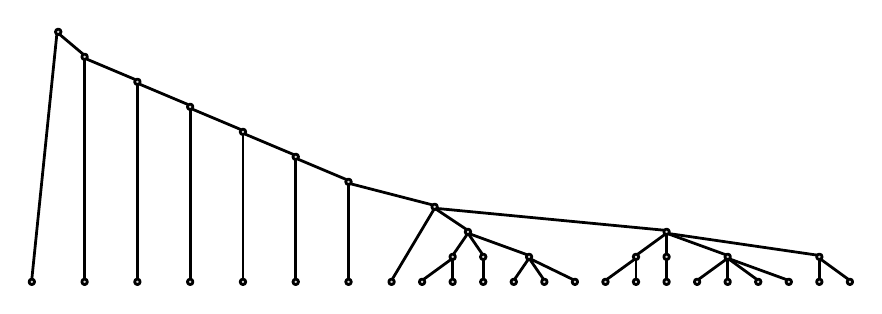
\begin{tikzpicture}[>=latex,line join=bevel,scale=0.5]
  \pgfsetlinewidth{1bp}
%%
\begin{scope}
  \pgfsetstrokecolor{black}
  \definecolor{strokecol}{rgb}{1.0,1.0,1.0};
  \pgfsetstrokecolor{strokecol}
  \definecolor{fillcol}{rgb}{1.0,1.0,1.0};
  \pgfsetfillcolor{fillcol}
  \filldraw (0bp,0bp) -- (0bp,184bp) -- (593bp,184bp) -- (593bp,0bp) -- cycle;
\end{scope}
\begin{scope}
  \pgfsetstrokecolor{black}
  \definecolor{strokecol}{rgb}{1.0,1.0,1.0};
  \pgfsetstrokecolor{strokecol}
  \definecolor{fillcol}{rgb}{1.0,1.0,1.0};
  \pgfsetfillcolor{fillcol}
  \filldraw (0bp,0bp) -- (0bp,184bp) -- (593bp,184bp) -- (593bp,0bp) -- cycle;
\end{scope}
\begin{scope}
  \pgfsetstrokecolor{black}
  \definecolor{strokecol}{rgb}{1.0,1.0,1.0};
  \pgfsetstrokecolor{strokecol}
  \definecolor{fillcol}{rgb}{1.0,1.0,1.0};
  \pgfsetfillcolor{fillcol}
  \filldraw (0bp,0bp) -- (0bp,184bp) -- (593bp,184bp) -- (593bp,0bp) -- cycle;
\end{scope}
\begin{scope}
  \pgfsetstrokecolor{black}
  \definecolor{strokecol}{rgb}{1.0,1.0,1.0};
  \pgfsetstrokecolor{strokecol}
  \definecolor{fillcol}{rgb}{1.0,1.0,1.0};
  \pgfsetfillcolor{fillcol}
  \filldraw (0bp,0bp) -- (0bp,184bp) -- (593bp,184bp) -- (593bp,0bp) -- cycle;
\end{scope}
\begin{scope}
  \pgfsetstrokecolor{black}
  \definecolor{strokecol}{rgb}{1.0,1.0,1.0};
  \pgfsetstrokecolor{strokecol}
  \definecolor{fillcol}{rgb}{1.0,1.0,1.0};
  \pgfsetfillcolor{fillcol}
  \filldraw (0bp,0bp) -- (0bp,184bp) -- (593bp,184bp) -- (593bp,0bp) -- cycle;
\end{scope}
\begin{scope}
  \pgfsetstrokecolor{black}
  \definecolor{strokecol}{rgb}{1.0,1.0,1.0};
  \pgfsetstrokecolor{strokecol}
  \definecolor{fillcol}{rgb}{1.0,1.0,1.0};
  \pgfsetfillcolor{fillcol}
  \filldraw (0bp,0bp) -- (0bp,184bp) -- (593bp,184bp) -- (593bp,0bp) -- cycle;
\end{scope}
\begin{scope}
  \pgfsetstrokecolor{black}
  \definecolor{strokecol}{rgb}{1.0,1.0,1.0};
  \pgfsetstrokecolor{strokecol}
  \definecolor{fillcol}{rgb}{1.0,1.0,1.0};
  \pgfsetfillcolor{fillcol}
  \filldraw (0bp,0bp) -- (0bp,184bp) -- (593bp,184bp) -- (593bp,0bp) -- cycle;
\end{scope}
\begin{scope}
  \pgfsetstrokecolor{black}
  \definecolor{strokecol}{rgb}{1.0,1.0,1.0};
  \pgfsetstrokecolor{strokecol}
  \definecolor{fillcol}{rgb}{1.0,1.0,1.0};
  \pgfsetfillcolor{fillcol}
  \filldraw (0bp,0bp) -- (0bp,184bp) -- (593bp,184bp) -- (593bp,0bp) -- cycle;
\end{scope}
\begin{scope}
  \pgfsetstrokecolor{black}
  \definecolor{strokecol}{rgb}{1.0,1.0,1.0};
  \pgfsetstrokecolor{strokecol}
  \definecolor{fillcol}{rgb}{1.0,1.0,1.0};
  \pgfsetfillcolor{fillcol}
  \filldraw (0bp,0bp) -- (0bp,184bp) -- (593bp,184bp) -- (593bp,0bp) -- cycle;
\end{scope}
\begin{scope}
  \pgfsetstrokecolor{black}
  \definecolor{strokecol}{rgb}{1.0,1.0,1.0};
  \pgfsetstrokecolor{strokecol}
  \definecolor{fillcol}{rgb}{1.0,1.0,1.0};
  \pgfsetfillcolor{fillcol}
  \filldraw (0bp,0bp) -- (0bp,184bp) -- (593bp,184bp) -- (593bp,0bp) -- cycle;
\end{scope}
\begin{scope}
  \pgfsetstrokecolor{black}
  \definecolor{strokecol}{rgb}{1.0,1.0,1.0};
  \pgfsetstrokecolor{strokecol}
  \definecolor{fillcol}{rgb}{1.0,1.0,1.0};
  \pgfsetfillcolor{fillcol}
  \filldraw (0bp,0bp) -- (0bp,184bp) -- (593bp,184bp) -- (593bp,0bp) -- cycle;
\end{scope}
\begin{scope}
  \pgfsetstrokecolor{black}
  \definecolor{strokecol}{rgb}{1.0,1.0,1.0};
  \pgfsetstrokecolor{strokecol}
  \definecolor{fillcol}{rgb}{1.0,1.0,1.0};
  \pgfsetfillcolor{fillcol}
  \filldraw (0bp,0bp) -- (0bp,184bp) -- (593bp,184bp) -- (593bp,0bp) -- cycle;
\end{scope}
\begin{scope}
  \pgfsetstrokecolor{black}
  \definecolor{strokecol}{rgb}{1.0,1.0,1.0};
  \pgfsetstrokecolor{strokecol}
  \definecolor{fillcol}{rgb}{1.0,1.0,1.0};
  \pgfsetfillcolor{fillcol}
  \filldraw (0bp,0bp) -- (0bp,184bp) -- (593bp,184bp) -- (593bp,0bp) -- cycle;
\end{scope}
\begin{scope}
  \pgfsetstrokecolor{black}
  \definecolor{strokecol}{rgb}{1.0,1.0,1.0};
  \pgfsetstrokecolor{strokecol}
  \definecolor{fillcol}{rgb}{1.0,1.0,1.0};
  \pgfsetfillcolor{fillcol}
  \filldraw (0bp,0bp) -- (0bp,184bp) -- (593bp,184bp) -- (593bp,0bp) -- cycle;
\end{scope}
\begin{scope}
  \pgfsetstrokecolor{black}
  \definecolor{strokecol}{rgb}{1.0,1.0,1.0};
  \pgfsetstrokecolor{strokecol}
  \definecolor{fillcol}{rgb}{1.0,1.0,1.0};
  \pgfsetfillcolor{fillcol}
  \filldraw (0bp,0bp) -- (0bp,184bp) -- (593bp,184bp) -- (593bp,0bp) -- cycle;
\end{scope}
\begin{scope}
  \pgfsetstrokecolor{black}
  \definecolor{strokecol}{rgb}{1.0,1.0,1.0};
  \pgfsetstrokecolor{strokecol}
  \definecolor{fillcol}{rgb}{1.0,1.0,1.0};
  \pgfsetfillcolor{fillcol}
  \filldraw (0bp,0bp) -- (0bp,184bp) -- (593bp,184bp) -- (593bp,0bp) -- cycle;
\end{scope}
\begin{scope}
  \pgfsetstrokecolor{black}
  \definecolor{strokecol}{rgb}{1.0,1.0,1.0};
  \pgfsetstrokecolor{strokecol}
  \definecolor{fillcol}{rgb}{1.0,1.0,1.0};
  \pgfsetfillcolor{fillcol}
  \filldraw (0bp,0bp) -- (0bp,184bp) -- (593bp,184bp) -- (593bp,0bp) -- cycle;
\end{scope}
\begin{scope}
  \pgfsetstrokecolor{black}
  \definecolor{strokecol}{rgb}{1.0,1.0,1.0};
  \pgfsetstrokecolor{strokecol}
  \definecolor{fillcol}{rgb}{1.0,1.0,1.0};
  \pgfsetfillcolor{fillcol}
  \filldraw (0bp,0bp) -- (0bp,184bp) -- (593bp,184bp) -- (593bp,0bp) -- cycle;
\end{scope}
  \pgfsetcolor{black}
  % Edge: c6 -> c7
  \draw [-] (116bp,125.94bp) -- (116bp,4.0576bp);
  % Edge: c14 -> c16
  \draw [-] (293.29bp,54.14bp) -- (314.82bp,39.788bp);
  % Edge: c2 -> c4
  \draw [-] (41.633bp,162.31bp) -- (76.416bp,147.67bp);
  % Edge: c23 -> c37
  \draw [-] (504.46bp,18.468bp) -- (545.49bp,3.5508bp);
  % Edge: c20 -> c30
  \draw [-] (361.42bp,18.312bp) -- (391.62bp,3.6671bp);
  % Edge: c24 -> c38
  \draw [-] (569bp,17.95bp) -- (569bp,4.0746bp);
  % Edge: c20 -> c28
  \draw [-] (359.28bp,17.95bp) -- (349.74bp,4.0746bp);
  % Edge: c17 -> c23
  \draw [-] (460.46bp,36.468bp) -- (501.49bp,21.551bp);
  % Edge: c4 -> c5
  \draw [-] (78bp,143.94bp) -- (78bp,4.0576bp);
  % Edge: root -> c2
  \draw [-] (22.022bp,180.14bp) -- (39.064bp,165.79bp);
  % Edge: c14 -> c17
  \draw [-] (293.88bp,54.82bp) -- (457.35bp,39.158bp);
  % Edge: c8 -> c9
  \draw [-] (154bp,107.94bp) -- (154bp,4.0576bp);
  % Edge: c23 -> c34
  \draw [-] (501.82bp,18.14bp) -- (482.08bp,3.788bp);
  % Edge: c23 -> c36
  \draw [-] (504.18bp,18.14bp) -- (523.92bp,3.788bp);
  % Edge: c12 -> c13
  \draw [-] (230bp,71.785bp) -- (230bp,4.037bp);
  % Edge: c6 -> c8
  \draw [-] (117.63bp,126.31bp) -- (152.42bp,111.67bp);
  % Edge: c20 -> c29
  \draw [-] (360.72bp,17.95bp) -- (370.26bp,4.0746bp);
  % Edge: c21 -> c32
  \draw [-] (437bp,17.95bp) -- (437bp,4.0746bp);
  % Edge: root -> c1
  \draw [-] (19.978bp,180.05bp) -- (2bp,4.0576bp);
  % Edge: c17 -> c24
  \draw [-] (460.91bp,36.722bp) -- (567.37bp,21.237bp);
  % Edge: c10 -> c11
  \draw [-] (192bp,89.942bp) -- (192bp,4.0576bp);
  % Edge: c4 -> c6
  \draw [-] (79.633bp,144.31bp) -- (114.42bp,129.67bp);
  % Edge: c12 -> c14
  \draw [-] (231.53bp,72.604bp) -- (290.29bp,57.44bp);
  % Edge: c23 -> c35
  \draw [-] (503bp,17.95bp) -- (503bp,4.0746bp);
  % Edge: c18 -> c26
  \draw [-] (305bp,17.95bp) -- (305bp,4.0746bp);
  % Edge: c8 -> c10
  \draw [-] (155.63bp,108.31bp) -- (190.42bp,93.667bp);
  % Edge: c17 -> c21
  \draw [-] (457.82bp,36.14bp) -- (438.08bp,21.788bp);
  % Edge: c16 -> c20
  \draw [-] (317.46bp,36.468bp) -- (358.49bp,21.551bp);
  % Edge: c22 -> c33
  \draw [-] (459bp,17.95bp) -- (459bp,4.0746bp);
  % Edge: c14 -> c15
  \draw [-] (291.23bp,53.715bp) -- (261.63bp,4.0623bp);
  % Edge: c16 -> c19
  \draw [-] (316.72bp,35.95bp) -- (326.26bp,22.075bp);
  % Edge: c18 -> c25
  \draw [-] (303.82bp,18.14bp) -- (284.08bp,3.788bp);
  % Edge: c2 -> c3
  \draw [-] (40bp,161.94bp) -- (40bp,4.0576bp);
  % Edge: c10 -> c12
  \draw [-] (193.63bp,90.312bp) -- (228.42bp,75.667bp);
  % Edge: c24 -> c39
  \draw [-] (570.18bp,18.14bp) -- (589.92bp,3.788bp);
  % Edge: c16 -> c18
  \draw [-] (315.28bp,35.95bp) -- (305.74bp,22.075bp);
  % Edge: c17 -> c22
  \draw [-] (459bp,35.95bp) -- (459bp,22.075bp);
  % Edge: c21 -> c31
  \draw [-] (435.82bp,18.14bp) -- (416.08bp,3.788bp);
  % Edge: c19 -> c27
  \draw [-] (327bp,17.95bp) -- (327bp,4.0746bp);
  % Node: c36
\begin{scope}
  \definecolor{strokecol}{rgb}{0.0,0.0,0.0};
  \pgfsetstrokecolor{strokecol}
  \definecolor{fillcol}{rgb}{0.83,0.83,0.83};
  \pgfsetfillcolor{fillcol}
  \filldraw [opacity=1] (525bp,2bp) ellipse (2bp and 2bp);
\end{scope}
  % Node: c37
\begin{scope}
  \definecolor{strokecol}{rgb}{0.0,0.0,0.0};
  \pgfsetstrokecolor{strokecol}
  \definecolor{fillcol}{rgb}{0.83,0.83,0.83};
  \pgfsetfillcolor{fillcol}
  \filldraw [opacity=1] (547bp,2bp) ellipse (2bp and 2bp);
\end{scope}
  % Node: c19
\begin{scope}
  \definecolor{strokecol}{rgb}{0.0,0.0,0.0};
  \pgfsetstrokecolor{strokecol}
  \definecolor{fillcol}{rgb}{0.83,0.83,0.83};
  \pgfsetfillcolor{fillcol}
  \filldraw [opacity=1] (327bp,20bp) ellipse (2bp and 2bp);
\end{scope}
  % Node: c18
\begin{scope}
  \definecolor{strokecol}{rgb}{0.0,0.0,0.0};
  \pgfsetstrokecolor{strokecol}
  \definecolor{fillcol}{rgb}{0.83,0.83,0.83};
  \pgfsetfillcolor{fillcol}
  \filldraw [opacity=1] (305bp,20bp) ellipse (2bp and 2bp);
\end{scope}
  % Node: c39
\begin{scope}
  \definecolor{strokecol}{rgb}{0.0,0.0,0.0};
  \pgfsetstrokecolor{strokecol}
  \definecolor{fillcol}{rgb}{0.83,0.83,0.83};
  \pgfsetfillcolor{fillcol}
  \filldraw [opacity=1] (591bp,2bp) ellipse (2bp and 2bp);
\end{scope}
  % Node: c38
\begin{scope}
  \definecolor{strokecol}{rgb}{0.0,0.0,0.0};
  \pgfsetstrokecolor{strokecol}
  \definecolor{fillcol}{rgb}{0.83,0.83,0.83};
  \pgfsetfillcolor{fillcol}
  \filldraw [opacity=1] (569bp,2bp) ellipse (2bp and 2bp);
\end{scope}
  % Node: c13
\begin{scope}
  \definecolor{strokecol}{rgb}{0.0,0.0,0.0};
  \pgfsetstrokecolor{strokecol}
  \definecolor{fillcol}{rgb}{0.83,0.83,0.83};
  \pgfsetfillcolor{fillcol}
  \filldraw [opacity=1] (230bp,2bp) ellipse (2bp and 2bp);
\end{scope}
  % Node: c12
\begin{scope}
  \definecolor{strokecol}{rgb}{0.0,0.0,0.0};
  \pgfsetstrokecolor{strokecol}
  \definecolor{fillcol}{rgb}{0.83,0.83,0.83};
  \pgfsetfillcolor{fillcol}
  \filldraw [opacity=1] (230bp,74bp) ellipse (2bp and 2bp);
\end{scope}
  % Node: c11
\begin{scope}
  \definecolor{strokecol}{rgb}{0.0,0.0,0.0};
  \pgfsetstrokecolor{strokecol}
  \definecolor{fillcol}{rgb}{0.83,0.83,0.83};
  \pgfsetfillcolor{fillcol}
  \filldraw [opacity=1] (192bp,2bp) ellipse (2bp and 2bp);
\end{scope}
  % Node: c10
\begin{scope}
  \definecolor{strokecol}{rgb}{0.0,0.0,0.0};
  \pgfsetstrokecolor{strokecol}
  \definecolor{fillcol}{rgb}{0.83,0.83,0.83};
  \pgfsetfillcolor{fillcol}
  \filldraw [opacity=1] (192bp,92bp) ellipse (2bp and 2bp);
\end{scope}
  % Node: c17
\begin{scope}
  \definecolor{strokecol}{rgb}{0.0,0.0,0.0};
  \pgfsetstrokecolor{strokecol}
  \definecolor{fillcol}{rgb}{0.83,0.83,0.83};
  \pgfsetfillcolor{fillcol}
  \filldraw [opacity=1] (459bp,38bp) ellipse (2bp and 2bp);
\end{scope}
  % Node: c16
\begin{scope}
  \definecolor{strokecol}{rgb}{0.0,0.0,0.0};
  \pgfsetstrokecolor{strokecol}
  \definecolor{fillcol}{rgb}{0.83,0.83,0.83};
  \pgfsetfillcolor{fillcol}
  \filldraw [opacity=1] (316bp,38bp) ellipse (2bp and 2bp);
\end{scope}
  % Node: c15
\begin{scope}
  \definecolor{strokecol}{rgb}{0.0,0.0,0.0};
  \pgfsetstrokecolor{strokecol}
  \definecolor{fillcol}{rgb}{0.83,0.83,0.83};
  \pgfsetfillcolor{fillcol}
  \filldraw [opacity=1] (261bp,2bp) ellipse (2bp and 2bp);
\end{scope}
  % Node: c14
\begin{scope}
  \definecolor{strokecol}{rgb}{0.0,0.0,0.0};
  \pgfsetstrokecolor{strokecol}
  \definecolor{fillcol}{rgb}{0.83,0.83,0.83};
  \pgfsetfillcolor{fillcol}
  \filldraw [opacity=1] (292bp,56bp) ellipse (2bp and 2bp);
\end{scope}
  % Node: c35
\begin{scope}
  \definecolor{strokecol}{rgb}{0.0,0.0,0.0};
  \pgfsetstrokecolor{strokecol}
  \definecolor{fillcol}{rgb}{0.83,0.83,0.83};
  \pgfsetfillcolor{fillcol}
  \filldraw [opacity=1] (503bp,2bp) ellipse (2bp and 2bp);
\end{scope}
  % Node: c9
\begin{scope}
  \definecolor{strokecol}{rgb}{0.0,0.0,0.0};
  \pgfsetstrokecolor{strokecol}
  \definecolor{fillcol}{rgb}{0.83,0.83,0.83};
  \pgfsetfillcolor{fillcol}
  \filldraw [opacity=1] (154bp,2bp) ellipse (2bp and 2bp);
\end{scope}
  % Node: c8
\begin{scope}
  \definecolor{strokecol}{rgb}{0.0,0.0,0.0};
  \pgfsetstrokecolor{strokecol}
  \definecolor{fillcol}{rgb}{0.83,0.83,0.83};
  \pgfsetfillcolor{fillcol}
  \filldraw [opacity=1] (154bp,110bp) ellipse (2bp and 2bp);
\end{scope}
  % Node: c34
\begin{scope}
  \definecolor{strokecol}{rgb}{0.0,0.0,0.0};
  \pgfsetstrokecolor{strokecol}
  \definecolor{fillcol}{rgb}{0.83,0.83,0.83};
  \pgfsetfillcolor{fillcol}
  \filldraw [opacity=1] (481bp,2bp) ellipse (2bp and 2bp);
\end{scope}
  % Node: c3
\begin{scope}
  \definecolor{strokecol}{rgb}{0.0,0.0,0.0};
  \pgfsetstrokecolor{strokecol}
  \definecolor{fillcol}{rgb}{0.83,0.83,0.83};
  \pgfsetfillcolor{fillcol}
  \filldraw [opacity=1] (40bp,2bp) ellipse (2bp and 2bp);
\end{scope}
  % Node: c2
\begin{scope}
  \definecolor{strokecol}{rgb}{0.0,0.0,0.0};
  \pgfsetstrokecolor{strokecol}
  \definecolor{fillcol}{rgb}{0.83,0.83,0.83};
  \pgfsetfillcolor{fillcol}
  \filldraw [opacity=1] (40bp,164bp) ellipse (2bp and 2bp);
\end{scope}
  % Node: c1
\begin{scope}
  \definecolor{strokecol}{rgb}{0.0,0.0,0.0};
  \pgfsetstrokecolor{strokecol}
  \definecolor{fillcol}{rgb}{0.83,0.83,0.83};
  \pgfsetfillcolor{fillcol}
  \filldraw [opacity=1] (2bp,2bp) ellipse (2bp and 2bp);
\end{scope}
  % Node: c7
\begin{scope}
  \definecolor{strokecol}{rgb}{0.0,0.0,0.0};
  \pgfsetstrokecolor{strokecol}
  \definecolor{fillcol}{rgb}{0.83,0.83,0.83};
  \pgfsetfillcolor{fillcol}
  \filldraw [opacity=1] (116bp,2bp) ellipse (2bp and 2bp);
\end{scope}
  % Node: c6
\begin{scope}
  \definecolor{strokecol}{rgb}{0.0,0.0,0.0};
  \pgfsetstrokecolor{strokecol}
  \definecolor{fillcol}{rgb}{0.83,0.83,0.83};
  \pgfsetfillcolor{fillcol}
  \filldraw [opacity=1] (116bp,128bp) ellipse (2bp and 2bp);
\end{scope}
  % Node: c5
\begin{scope}
  \definecolor{strokecol}{rgb}{0.0,0.0,0.0};
  \pgfsetstrokecolor{strokecol}
  \definecolor{fillcol}{rgb}{0.83,0.83,0.83};
  \pgfsetfillcolor{fillcol}
  \filldraw [opacity=1] (78bp,2bp) ellipse (2bp and 2bp);
\end{scope}
  % Node: c4
\begin{scope}
  \definecolor{strokecol}{rgb}{0.0,0.0,0.0};
  \pgfsetstrokecolor{strokecol}
  \definecolor{fillcol}{rgb}{0.83,0.83,0.83};
  \pgfsetfillcolor{fillcol}
  \filldraw [opacity=1] (78bp,146bp) ellipse (2bp and 2bp);
\end{scope}
  % Node: c22
\begin{scope}
  \definecolor{strokecol}{rgb}{0.0,0.0,0.0};
  \pgfsetstrokecolor{strokecol}
  \definecolor{fillcol}{rgb}{0.83,0.83,0.83};
  \pgfsetfillcolor{fillcol}
  \filldraw [opacity=1] (459bp,20bp) ellipse (2bp and 2bp);
\end{scope}
  % Node: c23
\begin{scope}
  \definecolor{strokecol}{rgb}{0.0,0.0,0.0};
  \pgfsetstrokecolor{strokecol}
  \definecolor{fillcol}{rgb}{0.83,0.83,0.83};
  \pgfsetfillcolor{fillcol}
  \filldraw [opacity=1] (503bp,20bp) ellipse (2bp and 2bp);
\end{scope}
  % Node: c20
\begin{scope}
  \definecolor{strokecol}{rgb}{0.0,0.0,0.0};
  \pgfsetstrokecolor{strokecol}
  \definecolor{fillcol}{rgb}{0.83,0.83,0.83};
  \pgfsetfillcolor{fillcol}
  \filldraw [opacity=1] (360bp,20bp) ellipse (2bp and 2bp);
\end{scope}
  % Node: c21
\begin{scope}
  \definecolor{strokecol}{rgb}{0.0,0.0,0.0};
  \pgfsetstrokecolor{strokecol}
  \definecolor{fillcol}{rgb}{0.83,0.83,0.83};
  \pgfsetfillcolor{fillcol}
  \filldraw [opacity=1] (437bp,20bp) ellipse (2bp and 2bp);
\end{scope}
  % Node: c26
\begin{scope}
  \definecolor{strokecol}{rgb}{0.0,0.0,0.0};
  \pgfsetstrokecolor{strokecol}
  \definecolor{fillcol}{rgb}{0.83,0.83,0.83};
  \pgfsetfillcolor{fillcol}
  \filldraw [opacity=1] (305bp,2bp) ellipse (2bp and 2bp);
\end{scope}
  % Node: c27
\begin{scope}
  \definecolor{strokecol}{rgb}{0.0,0.0,0.0};
  \pgfsetstrokecolor{strokecol}
  \definecolor{fillcol}{rgb}{0.83,0.83,0.83};
  \pgfsetfillcolor{fillcol}
  \filldraw [opacity=1] (327bp,2bp) ellipse (2bp and 2bp);
\end{scope}
  % Node: c24
\begin{scope}
  \definecolor{strokecol}{rgb}{0.0,0.0,0.0};
  \pgfsetstrokecolor{strokecol}
  \definecolor{fillcol}{rgb}{0.83,0.83,0.83};
  \pgfsetfillcolor{fillcol}
  \filldraw [opacity=1] (569bp,20bp) ellipse (2bp and 2bp);
\end{scope}
  % Node: c25
\begin{scope}
  \definecolor{strokecol}{rgb}{0.0,0.0,0.0};
  \pgfsetstrokecolor{strokecol}
  \definecolor{fillcol}{rgb}{0.83,0.83,0.83};
  \pgfsetfillcolor{fillcol}
  \filldraw [opacity=1] (283bp,2bp) ellipse (2bp and 2bp);
\end{scope}
  % Node: c31
\begin{scope}
  \definecolor{strokecol}{rgb}{0.0,0.0,0.0};
  \pgfsetstrokecolor{strokecol}
  \definecolor{fillcol}{rgb}{0.83,0.83,0.83};
  \pgfsetfillcolor{fillcol}
  \filldraw [opacity=1] (415bp,2bp) ellipse (2bp and 2bp);
\end{scope}
  % Node: c28
\begin{scope}
  \definecolor{strokecol}{rgb}{0.0,0.0,0.0};
  \pgfsetstrokecolor{strokecol}
  \definecolor{fillcol}{rgb}{0.83,0.83,0.83};
  \pgfsetfillcolor{fillcol}
  \filldraw [opacity=1] (349bp,2bp) ellipse (2bp and 2bp);
\end{scope}
  % Node: c29
\begin{scope}
  \definecolor{strokecol}{rgb}{0.0,0.0,0.0};
  \pgfsetstrokecolor{strokecol}
  \definecolor{fillcol}{rgb}{0.83,0.83,0.83};
  \pgfsetfillcolor{fillcol}
  \filldraw [opacity=1] (371bp,2bp) ellipse (2bp and 2bp);
\end{scope}
  % Node: c30
\begin{scope}
  \definecolor{strokecol}{rgb}{0.0,0.0,0.0};
  \pgfsetstrokecolor{strokecol}
  \definecolor{fillcol}{rgb}{0.83,0.83,0.83};
  \pgfsetfillcolor{fillcol}
  \filldraw [opacity=1] (393bp,2bp) ellipse (2bp and 2bp);
\end{scope}
  % Node: c33
\begin{scope}
  \definecolor{strokecol}{rgb}{0.0,0.0,0.0};
  \pgfsetstrokecolor{strokecol}
  \definecolor{fillcol}{rgb}{0.83,0.83,0.83};
  \pgfsetfillcolor{fillcol}
  \filldraw [opacity=1] (459bp,2bp) ellipse (2bp and 2bp);
\end{scope}
  % Node: c32
\begin{scope}
  \definecolor{strokecol}{rgb}{0.0,0.0,0.0};
  \pgfsetstrokecolor{strokecol}
  \definecolor{fillcol}{rgb}{0.83,0.83,0.83};
  \pgfsetfillcolor{fillcol}
  \filldraw [opacity=1] (437bp,2bp) ellipse (2bp and 2bp);
\end{scope}
  % Node: root
\begin{scope}
  \definecolor{strokecol}{rgb}{0.0,0.0,0.0};
  \pgfsetstrokecolor{strokecol}
  \definecolor{fillcol}{rgb}{0.83,0.83,0.83};
  \pgfsetfillcolor{fillcol}
  \filldraw [opacity=1] (21bp,182bp) ellipse (2bp and 2bp);
\end{scope}
%
\end{tikzpicture}


\end{center}
\caption{A badly-drawn multiple-outlier cover tree.}
\label{fig:outliers}
\end{figure}

A tree that has this chain-like structure all the way down is going to perform
horrendously; motivated by this observation, we define a measure of tree
imbalance.

\begin{defn}
The {\it cover node imbalance} $i_n(\mathscr{N}_i)$ for a cover tree node
$\mathscr{N}_i$ with scale $s_i$ in the cover tree $\mathscr{T}$ is defined as
the cumulative number of missing levels between the node and its parent
$\mathscr{N}_p$ (which has scale $s_p$).  If
the node is a leaf child (that is, $s_i = -\infty$), then number of missing
levels is defined as the difference between $s_p$ and $s_{\min} - 1$ where
$s_{\min}$ is the smallest scale of a non-leaf node in $\mathscr{T}$.  If
$\mathscr{N}_i$ is the root of the tree, then the cover node imbalance is 0.
Explicitly written, this calculation is

\begin{equation}
i_n(\mathscr{N}_i) = \begin{dcases*}
  s_p - s_i - 1 & if $\mathscr{N}_i$ is not a leaf and not the root node \\
  \max(s_p - s_{\min} - 1, \; 0) & if $\mathscr{N}_i$ is a leaf \\
  0 & if $\mathscr{N}_i$ is the root node.
  \end{dcases*}
\end{equation}
\end{defn}

This simple definition of cover node imbalance is easy to calculate, and using
it, we can generalize to a measure of imbalance for the full tree.

\begin{defn}
The {\it cover tree imbalance} $i_t(\mathscr{T})$ for a cover tree $\mathscr{T}$
is defined as the cumulative number of missing levels in the tree.  This can be
expressed as a function of cover node imbalances easily:

\begin{equation}
i_t(\mathscr{T}) = \sum_{\mathscr{N}_i \in \mathscr{T}} i_n(\mathscr{N}_i).
\end{equation}
\end{defn}

A perfectly balanced cover tree $\mathscr{T}_b$ with no missing levels has
imbalance $i_t(\mathscr{T}_b) = 0$ (for instance, Figure
\ref{fig:imbalance-good}).  A worst-case cover tree $\mathscr{T}_w$ which is
entirely a chain-like structure with maximum scale $s_{\max}$ and minimum scale
$s_{\min}$ will have imbalance $i_t(\mathscr{T}_w) \sim N (s_{\max} -
s_{\min})$.  Because of this chain-like structure, each level has only one node
and thus there are at least $N$ levels; or, $s_{\max} - s_{\min} \ge N$, meaning
that the imbalance is actually quadratic in $N$!

As we will see later empirically, the notion of cover tree imbalance does a good
job of capturing the `goodness' of a tree.  We will use this notion in order to
quantify the worst-case performance of dual-tree algorithms using the cover
tree.

{\bf TODO: Can any bound be proven on $i_t(\mathscr{T})$?  I haven't thought of
anything successfully yet.}
